\section{IMPLEMENTATION} % (MAXIMUM 6 PAGES) 
\label{sec:implementation}
\begin{figure}[h!]
  \begin{center}
    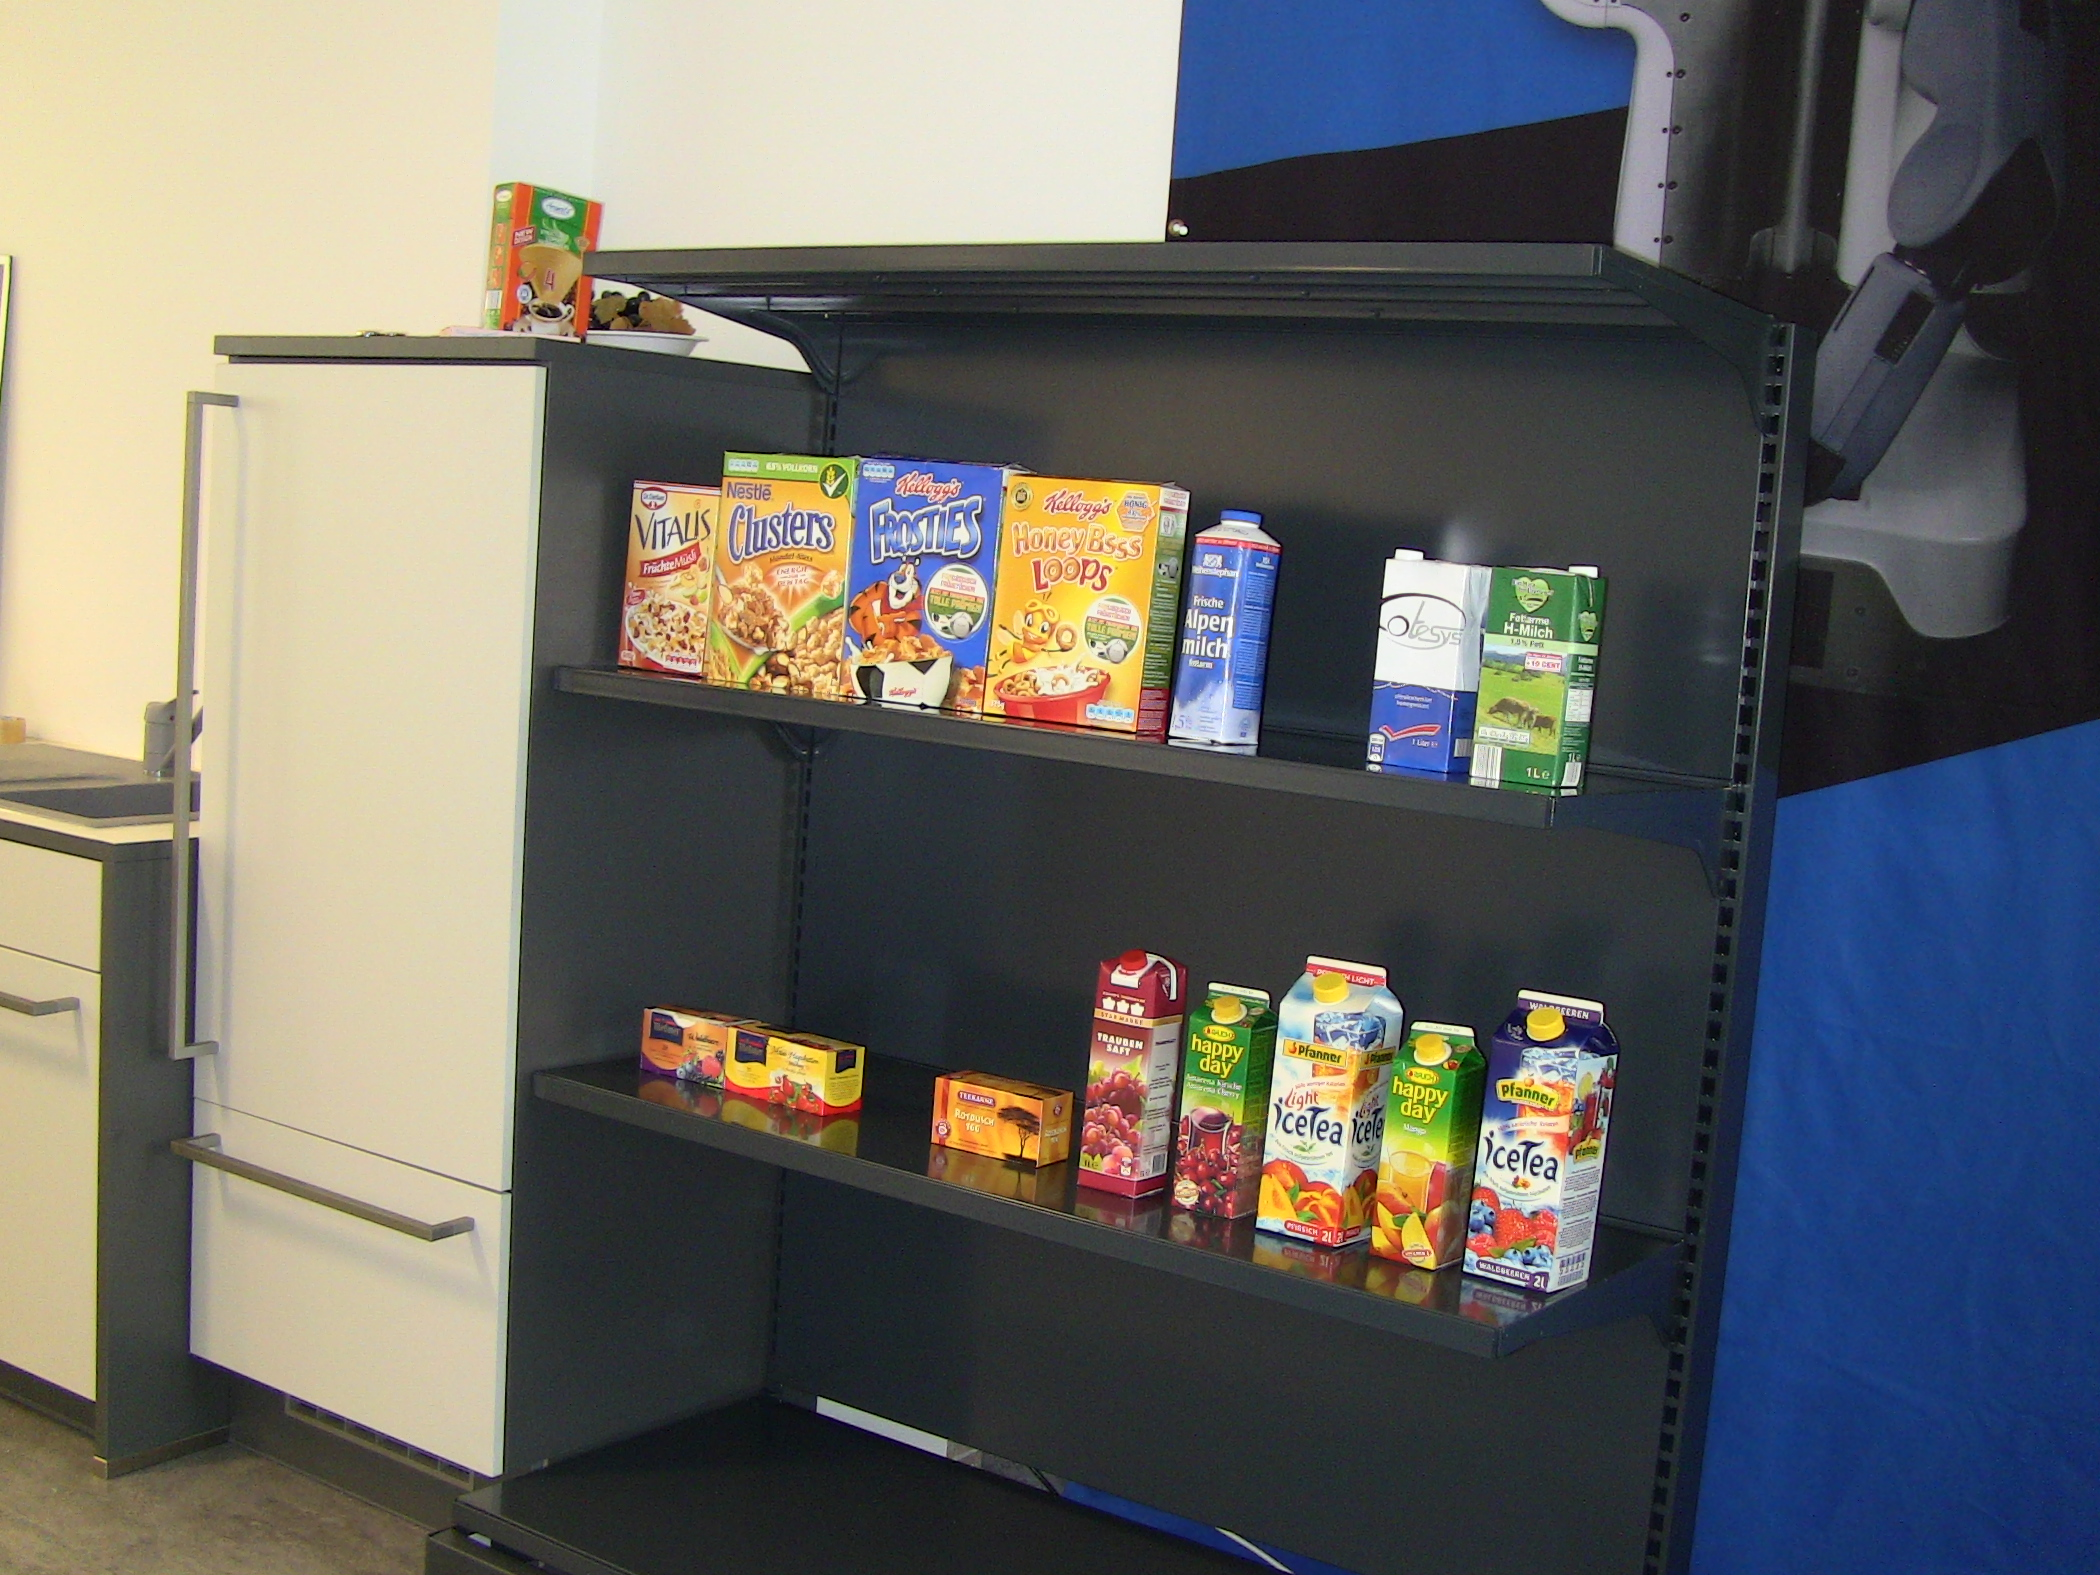
\includegraphics[width=0.25\textwidth]
    {figures/storage_rack.JPG}
    {\large$\rightarrow$}
    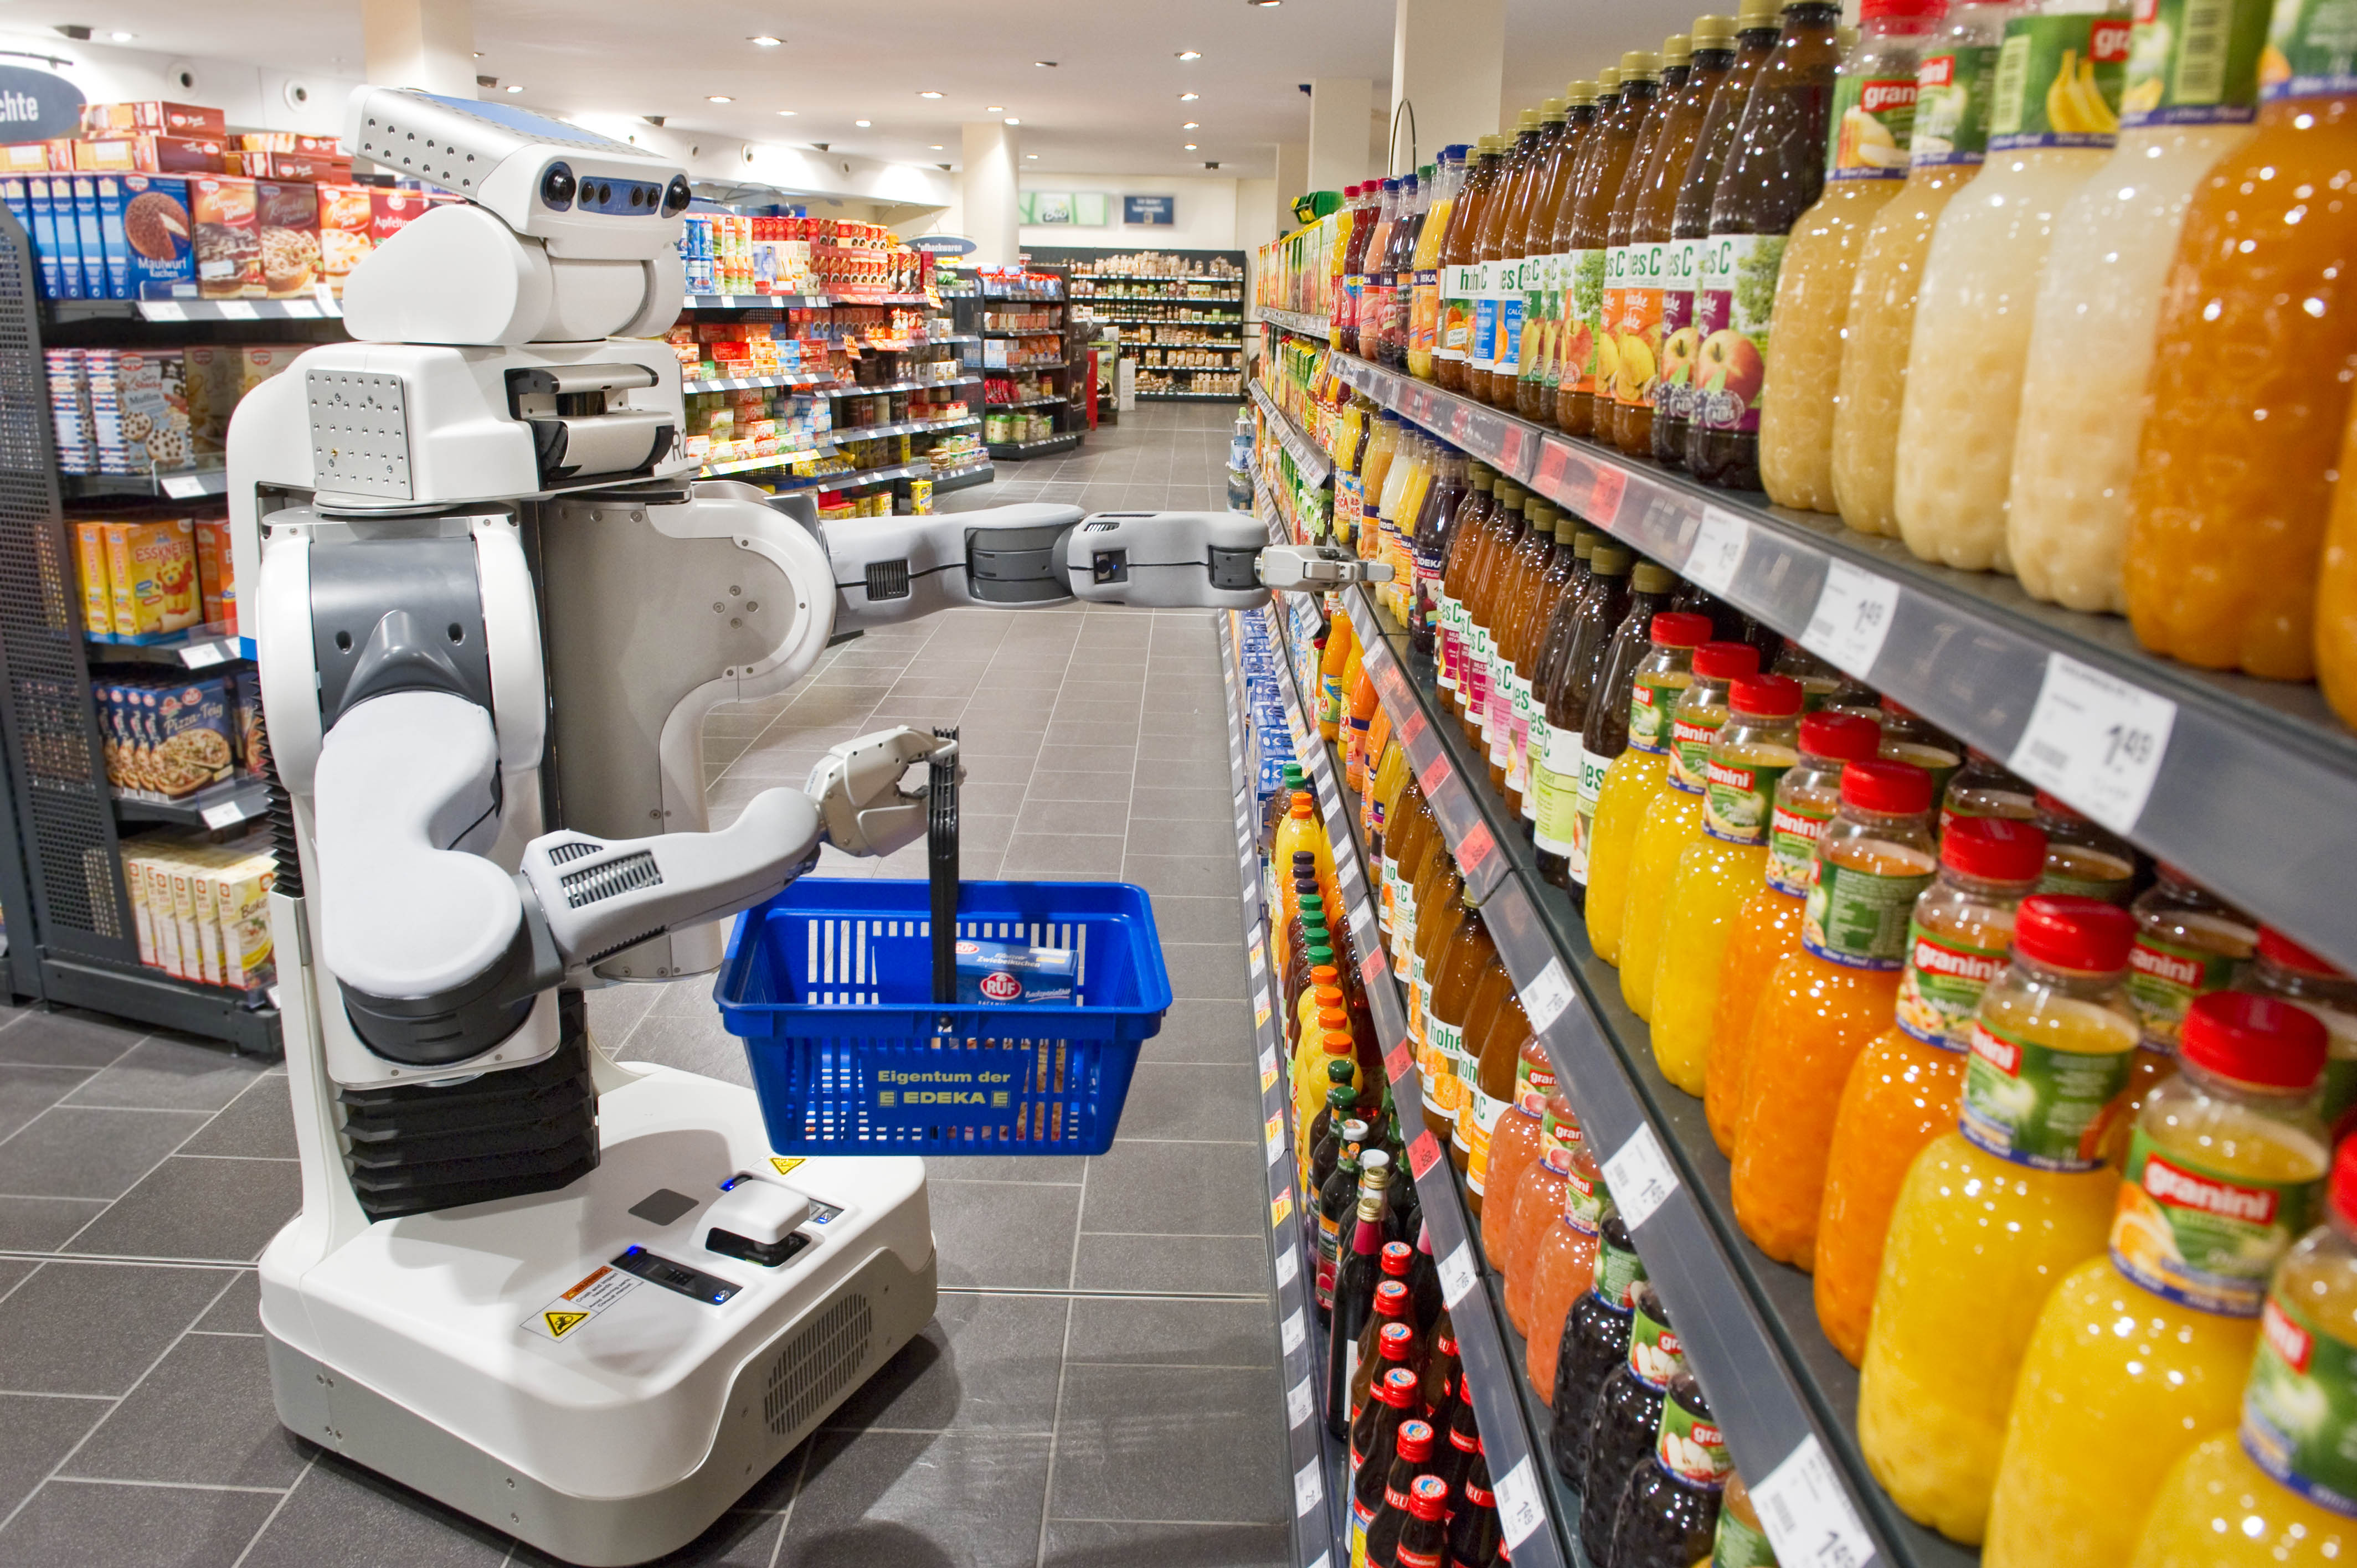
\includegraphics[width=0.25\textwidth]
    {figures/pr2_edeka_basket_1.jpg}
    {\large$\rightarrow$}
    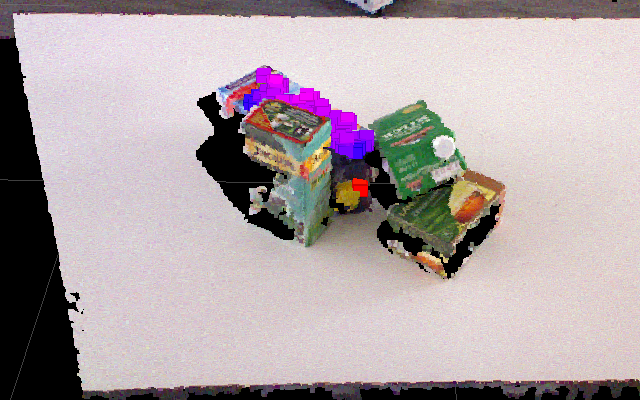
\includegraphics[width=0.25\textwidth]
    {figures/clutter-objects.png} \\
    % {\large$\rightarrow$}
    % \includegraphics[width=0.25\textwidth]
    % {mapping/clutter/basket_flipped.jpg}\\
    \vspace{2ex}
    
\includegraphics[width=0.25\textwidth]
    {figures/all_segmented.png}
    {\large$\rightarrow$}
    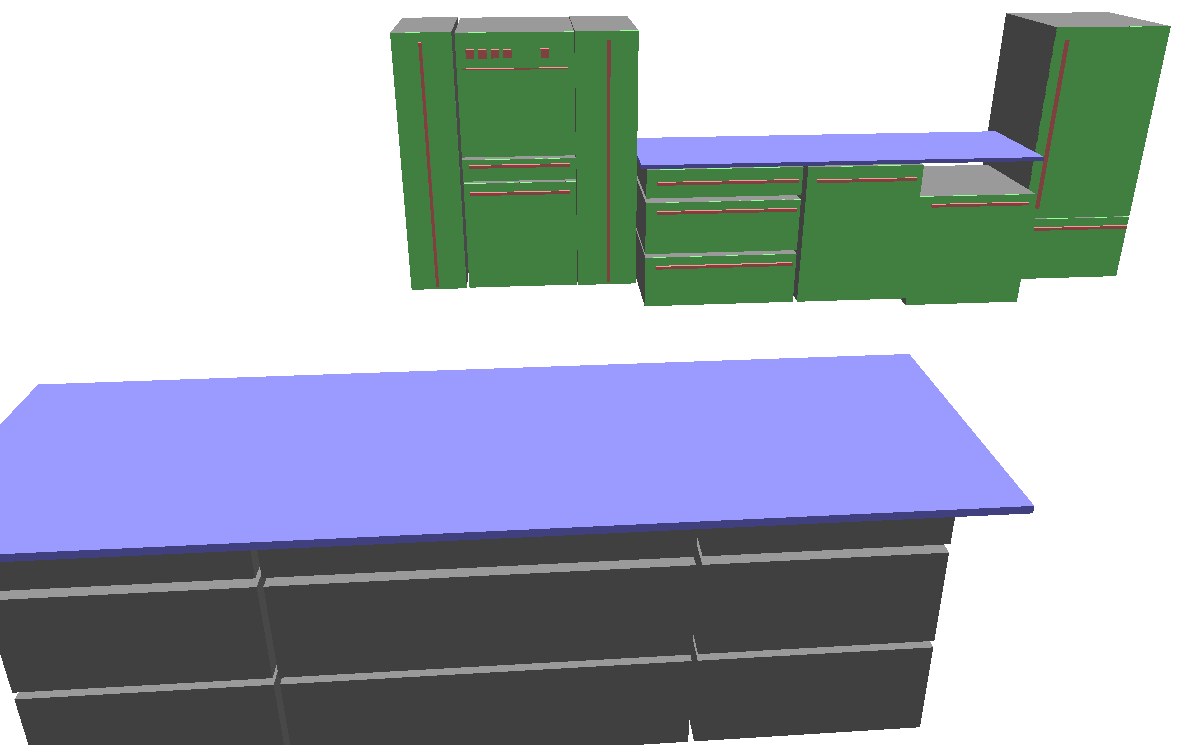
\includegraphics[width=0.25\textwidth]{figures/xml_map.png}
    {\large$\rightarrow$}
    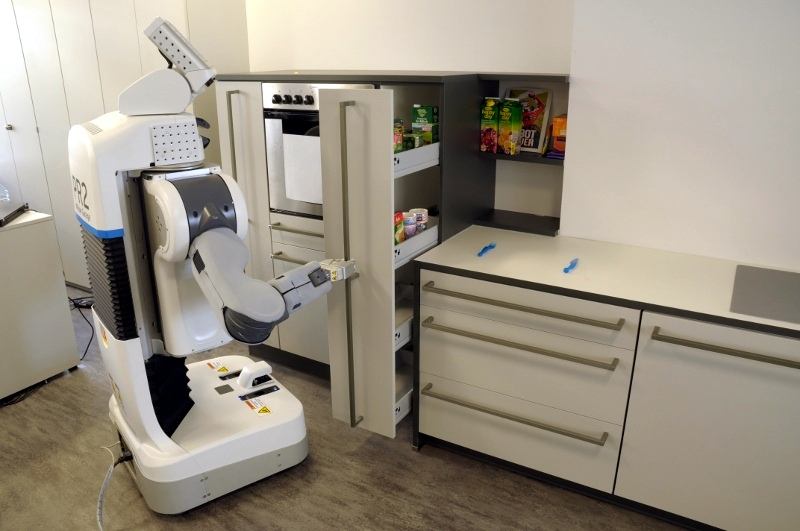
\includegraphics[width=0.25\textwidth]
    {figures/pr2_highdrawer.jpg}
  \end{center}
  \caption{\small{Robot simulating a shopping task and making use of \ksem\ generated semantic object map. \textbf{Top-left, top-middle:} 
    typical objects and scenes that robot is to perceive and manipulate using mechanisms from \ksem. 
    \textbf{Top-right:} recognition and pose detection of objects in cluttered scenes. \textbf{Bottom-left, bottom-middle:} 
  3D-based environment reconstruction and static world modeling. \textbf{Bottom-right:} Robot learns typical storage locations
using e.g. WUP~\cite{wup} similarities and places the object where it belongs to.}}
  \label{fig:teaser}
\end{figure}
\subsection{Quality of infrastructure / facilities and international collaboration of host} 
\subsubsection{Berkeley}
Berkeley's Department of  Electrical Engineering and Computer Sciences
(EECS) offers one of the strongest research and instructional programs
in this field anywhere in the world. The key strengths of the outgoing
host  lie in  the integration  of fundamental  theoretical  ideas with
practical applications, leading to a wide range of cross-disciplinary,
collaborative projects. The  integration of electrical engineering and
computer science forms the  core, with strong interactions that extend
into biological  sciences, mechanical and  civil engineering, physical
sciences,  chemistry,  mathematics,   operations  research,  etc.  The
programs have been consistently ranked in the top three in the USA and
worldwide by various organizations that rank academic programs.

Each year, top  students from all parts of the  world are attracted to
Berkeley by the excellence of  the faculty, the breadth of educational
opportunities   in   EECS    and   campus-wide,   and   the   Berkeley
environment. The  department's close ties to industry,  coupled to its
commitment to engineering research and education, ensure that students
get  a rigorous,  relevant, and  broad education.  Faculty  members at
Berkeley are committed to research and discovery at the highest level,
informed and creative teaching, and  the creative desire to excel. The
distinction of the EECS faculty has  been recognized in a long list of
prestigious honors and awards, including 2 National Medals of Science,
3 ACM  Turing Awards, 3 IEEE Medals  of Honor, and the  election of 37
faculty to the National  Academy of Engineering. The Department's list
of active  teaching faculty members  includes 7 winners of  the Campus
Distinguished Teaching Award.

The EECS  Center for Student Affairs  (CSA) plays a major  role in the
lives of more  than 1000 undergraduate and 500  graduate students - it
offers  a   wide  range  of  administrative,   academic  and  referral
services. Supplementing this  institutional support for students, more
than   15  EECS   student  organizations   and  over   30  campus-wide
organizations  support   their  students   on  their  journey   here  at
Berkeley.  Finally, the  diversity of  its student  body  reflects their
commitment  that diversity enhances  education for  everyone, enriches
their culture, and strengthens their economy.

Prof. Goldberg and Prof. Abbeel have remarkable cooperations both on national
and international level (mostly in Europe and Japan). They have both published 
extensively and have between them over 10 registered patents. 

Berkeley's EECS department is as well as IAS at TUM among the recipients
of a PR2 robot and thus part of the PR2 Beta Program Community. 
Having the
same type of the robot on both sides will thus be essential for \ksem\ project.
The PR2 platform at Berkeley is physically located on the 7th floor of 
Sutardja Dai Hall---which also houses offices and lab
space of Prof. Abbeel and Prof. Goldberg. In addition to the PR2 robot,
the EECS department also makes several high-performance computing
clusters available for faculty and graduate student use, which include 
more than 1000 state-of-the-art CPUs connected by gigabit ethernet and 
terabytes of fast storage for research data and results. Amazon's EC2 is also
commonly used when additional computational power is required.
Additional equipment includes PhaseSpace MoCap, Vicon MoCap (2x),
4 SensAble Technologies Phantom Omni haptice devices, open space for
PR2 in which the test environments for \ksem\ project will be set up.

\subsubsection{TUM}
In  recent years, the  Technische Universit\"at  M\"unchen (TUM)  has been
consistently ranked the top academic institution in Germany in several
independent rankings. It provides an excellent environment (likely the
best  in  Germany) by  substantial  funding  from  the Bavarian  state
government,   the  German  government   and  many   private  companies
alike.  One   of  the   missions  of  the   university  is   to  boost
interdisciplinary  research   across  engineering,  natural  sciences,
medicine, and  humanities. Today the  TUM comprises 13  faculties with
more than 23,000  students (about 20 percent of  whom come from abroad
shows the degree of internationalization), 420 professors, and roughly
6,500 academic  and non-academic staff. The TUM is thus well
positioned  to create  new knowledge  and know-how  in Europe  and the
world.  In  2005  the  federal  and  state  governments  started  the
so-called Excellence Initiative in Germany. Between 2006 and 2011 they
will  fund the expansion  of top  university research  with up  to 1.9
billion Euros in three  funding categories: graduate schools, clusters
of excellence  and institutional strategies for  universities. The TUM
was recognized as  one of the first three  universities that succeeded
in   all   three  categories.    The   corporate   concept  ``TUM   The
Entrepreneurial  University'' supports  and advances  the  existing TUM
strategy and  promotes top-level research on multiple  levels. In this
context Entrepreneurial  Spirit means  to activate the  diversity of
human talent  in a concerted,  interactive way. In terms  of top-level
research, it entails combining a  maximum of individual freedom with a
supportive administration.

The proposed returning host  is the TUM Intelligent Autonomous Systems
Group (IAS~\footnote{http://ias.cs.tum.edu/}) from Professor Michael  
Beetz in the Munich city center, and its extension of the Munich Garching 
Campus. IAS consists of two  full-time   professors,  1  Junior  
Research   Group  Leader,  15 graduate  students, 2  secretaries.  This  very dynamic  group challenges
successfully  seven  main  research  topics: Perception  for  Robots;
Knowledge Processing; Plan-based Control; Cognitive Manipulation; 
Perception of  Human Activities; Facial Expression Recognition.
Its graduate  students co-supervise student projects and  nurture a solid
number of workshops  and seminars in German and  English, ranging from
ROS technologies, Knowledge Representation for Autonomous Robots (IROS
2011   Workshop  for   example),   to  3D   Perception  in   Robotics,
Cognition-enabled Mobile Manipulation  and up to Probabilistic Methods
for Perceiving, Learning and Reasoning about Everyday Activities~\footnote{http://ias.cs.tum.edu/events}. 
The group has  extended contacts  with the industry,  as evidenced  by the
number of student  placements in companies in Munich  and elsewhere in
Bavaria, and the ongoing research collaborations with major players in
the domain. In particular  in the robotics field,  with companies
such  as Kuka  GmbH, Aldebaran  Robotics, Willow Garage, Robert Bosch LLC  
and others.   The solid  and excellent  student basis  allows  this group  
to  further develop  its scientific path and  will give the applicant upon 
his return  to TUM the possibility of enriching his skills (in research, 
technology transfer, teaching and training).  In  this  context,   the applicant  
will  benefit  from  the  existing infrastructure  to  deliver thriving  
seminar  courses  to a  talented
student body. The  recently established international CoTeSys Graduate
School  (2010) will  extend  its activities  with  the development  of
specific  additional  measures  to  qualify  the  next  generation  of
graduate students, which  the applicant will contribute to supervise  and train.  The
returning  host  IAS has  extended  research academic  collaborations
abroad (USA, Japan, South-Korea, Europe),  which is a key asset in the
context of this  IOF proposal, as the applicant will be  called upon to contribute
to the reinforcement of scientific  and student exchanges with the USA
and Berkeley.
Prof.  Beetz,  IAS  Director,   is  additionally  a  member  and  the
vice-coordinator of the CoTeSys  Cluster of Excellence~\footnote{http://www.cotesys.org/} 
coordinated by TUM.  In CoTeSys there is a  close collaboration  between  scientists from  various
disciplines    connecting    neuro-cognitive   and    neuro-biological
foundations to  engineering sciences at  leading research institutions
in  Munich: besides  Technische Universit\"at  M\"unchen,  scientists from
Ludwig-Maximilians-Universit\"at   M\"unchen   -   LMU,  Universit\"at   der
Bundeswehr, Max-Planck Institute  of Neurobiology and German Aerospace
Agency  DLR are involved. CoTeSys
investigates cognition for technical systems such as vehicles, robots,
and   factories.  Cognitive  technical   systems  are   equipped  with
artificial  sensors  and   actuators,  integrated  and  embedded  into
physical  systems, and  act in  the physical  world. They  differ from
other technical systems since  they perform cognitive control and have
cognitive   capabilities.   By   cognitive  capabilities   they   mean
information processing that take into accounts: perception, attention,
memory,  action, learning,  and planning.  The  aim of  CoTeSys is  to
produce future  innovations.  This will  represent another opportunity
for applicant to diversify his activities and find additional partners for R\&D
projects  (whether academic  and local,  or industrial  and  spread in
Europe).

The equipment that is required for the realization of the project at the 
return host organization is already available. In
particular, three robot manipulation platforms -- a PR2\footnote{\url{http://www.willowgarage.com/pages/pr2}}, an
iCub\footnote{\url{http://www.robotcub.org}} and a custom-built robot
with KUKA lightweight arms and DLR/HIT hands -- are available for
real-world experiments on a daily basis. So is the testbed kitchen environment with an ample
set of ubiquitous devices such as Kinect sensors, ceiling cameras, RFID readers, etc.
\subsection{Practical arrangements for the implementation and 
management of the research project } 
\subsubsection{Berkeley}
Prof. Goldberg and Prof. Abbeel at Berkeley will reserve an office for the 
applicant with all the necessary equipment (computer, phone, internet access, 
secured access to the department IT network, e-mail account, access to laboratories).
A first working year plan will be defined in the first two weeks of the arrival. 
It will be formally revised at month 12. The applicant will be able to count on 
the support  of the accountant an secretary services. The applicant will be given 
assistance for the purchasing policy and the travel reimbursements claims.
\subsubsection{TUM}
The applicant will be inserted in the robust management structure of the IAS group. 
Applicant's direct connection with Prof. Michael Beetz, enriched by his interaction 
and supervision of undergraduate and graduate students  will ensure the success of the project. \\
\emph{Grant implementation:}\\
Eric Bourguignon  (CoTeSys Proposal Manager), who  has been associated
to the  non-scientific writing of  this proposal, will deliver  a
set of Marie-Curie FP7  tools to manage the  project, based on
his long-years experience  of EU grants management in  the FP6 and FP7
programs. The tools to be developed specifically for the projects will
include the  basic synopsis of  all contractual issues related  to the
project,  the  yearly reporting  ready-to-use  templates (science  and
finance) and regular follow-up meetings  with the applicant and the group 
team to ensure  a quality  delivery of  the expected  results.  The management
style will aim  at letting as much autonomy  in the budget controlling
to the applicant as possible. Both  administrative staff members, Mrs. Walter and
Mrs. Wagner, will take their load  to ensure the smooth running of the
project.

\emph{IAS investments on this project:}\\
It is estimated  that Prof. Beetz will spend  1,5 person-month on this
project on the 36 months of  the project duration. The IAS will lead
regular  reviewing of the  project. Applicant's re-integration
in  year  3  will  be  facilitated  by his  current  knowledge  of  the
University  structure,  its people,  its  finance and  its other  support
services.

%\todo{coordination btw TUM and Berkeley}
% From their  arrival, through the search of  national and international
% funding programs to the development and the promotion of new projects,
% the recruited  TUM scientists receive  high quality services  from the
% University,  e.g.   from  TUM  Office  for   Research  and  Innovation
% (TUM-Forte),  the  Welcome Office,  the  TUM Corporate  Communications
% Centre and  the TUM Patent and  License Office. Applicant knows  them, 
% and will re-learn quickly how to interact with them.

A strong involvement from the applicant's side will be expected in the design
and  monitoring  the organization   of  workshops at  major international
conferences. It is planned to organize 3 workshops in next 3 years, 1 at each of the
following conferences: ICRA, IROS and one machine learning conference. The applicant  will  coordinate  teams of
students  to  ensure  that  these  events are  successful.   From  the
beginning,  the applicant will fully  dispose his  travel budget  to attend
international  high-level conferences  as well  as to  develop  his own
scientific  network  and scientific  partnerships.   The applicant will  supervise
graduate and undergraduate students.

All details  have been agreed in  common with Prof. Goldberg and Prof. Abbeel  
at Berkeley and Prof. Beetz at TUM, during the preparation of this project proposal.

\subsection{Feasibility and credibility of the project, including work plan} 
%\todo{describe the table a bit, why tasks in paralles, training not in batches, etc}
In Sections~\ref{sec:q1} and~\ref{sec:q2} we detailed the three tasks to be carried 
out in this project, including the research methodology and the expected results. 
In Table~\ref{tab:timeplan} below the work plan is presented including the three 
work packages, plus two additional extra tasks for the integration of the developed systems
and the applicant's training, and we assigned an approximate time schedule for each of them.
The actual implementation steps are given in Section~\ref{sec:q2}. Certain tasks, such as e.g.
KSOM-Perception2 - KSOM-Perception4 will run in parallel as supervised student projects. 
For the workshops and the summer school the applicant reserved 1 week since the they will 
indeed take place at the week-long conferences which the applicant will attend in full.
The allocated time for applicant's training (soft skills and professional lectures, seminars)
is up to 4 weeks over the whole year. Regarding a risk analysis, the applicant plans to re-asses 
the goals set in the workplan in Table~\ref{tab:timeplan} every 6 months and report 
any changes back to the funding agency.   

A ``Partnership  Agreement'' will  be signed between  both institutions,
based on the existing Kowi model~\footnote{\url{http://www.kowi.de/Portaldata/2/Resources/fp7/marie-curie/FP7-MC-IOF-PartnershipAgreement-FINAL.pdf}}. This classical  agreement used  with many  Marie-Curie  fellowships, covers
also   Intellectual   Property   Rights   with  the   following
solution: ``If  the  results arise  from  collaborative efforts,  joint
ownership may be  negotiated. If this is the  case, PARTIES shall seek
to agree  amongst themselves arrangements for  applying for, obtaining
and/or maintaining such right on  a case-by-case basis. The same shall
apply for use and licensing such right. In case of a commercial use by
a  PARTY   or  licensing  to  third   parties,  appropriate  financial
compensation shall be given to the other PARTY concerned.''


\begin{table}[h!]
  \begin{Timeplan}
    % ---------------------------------------------------------------------
    % Representations
    % ---------------------------------------------------------------------
    \TimeplanChapter{\ksem\ Representation}
    \TimeplanRule{\ksem-Representation1 OWL}{0}{24}
    \hline
    \TimeplanRule{\ksem-Representation2 Scenes}{0}{30}
    \hline
    \TimeplanRule{\ksem-Representation3 Action-related}{12}{24}
    \hline
    % \TimeplanRule{\ksem-Rep4 First-order}{24}{12}
    % \hline
    
    % ---------------------------------------------------------------------
    % Perception
    % ---------------------------------------------------------------------
    \TimeplanChapter{\ksem\ Perception}
    \TimeplanRule{\ksem-Perception1 Infrastructure}{0}{18}
    \hline
    \TimeplanRule{\ksem-Perception2 Objects}{0}{24}
    \hline
    \TimeplanRule{\ksem-Perception3 Scenes}{0}{24}
    \hline
    \TimeplanRule{\ksem-Perception4 States}{0}{24}
    \hline
    % \TimeplanRule{\ksem-Per4 Activities}{24}{12}
    % \hline
    
    % ---------------------------------------------------------------------
    % Learning
    % ---------------------------------------------------------------------
    \TimeplanChapter{\ksem\ Acquisition and Learning}
    \TimeplanRule{\ksem-Learning1 Grounding}{0}{18}
    \hline
    \TimeplanRule{\ksem-Learning2 Locations}{3}{24}
    \hline
    \TimeplanRule{\ksem-Learning3 Relations}{6}{24}
    \hline
    \TimeplanRule{\ksem-Learning4 Lifelong}{18}{18}
    \hline
    
    % ---------------------------------------------------------------------
    % Integration, Documentation
    % ---------------------------------------------------------------------
    \TimeplanChapter{Integration, Evaluation and Documentation, Workshops, Summer School}
    \parbox[t]{\CaptionWidth}{\raggedright System integration\\*[0.1cm]} &
    \hspace*{9\MonthWidth}\rule{3\MonthWidth}{1.0ex}
    \hspace*{8.65\MonthWidth}\rule{3\MonthWidth}{1.0ex}
    \hspace*{8.65\MonthWidth}\rule{3\MonthWidth}{1.0ex}\\
    \hline
    \parbox[t]{\CaptionWidth}{\raggedright Evaluation, documentation\\*[0.1cm]} &
    \hspace*{9\MonthWidth}\rule{3\MonthWidth}{1.0ex}
    \hspace*{8.65\MonthWidth}\rule{3\MonthWidth}{1.0ex}
    \hspace*{8.65\MonthWidth}\rule{3\MonthWidth}{1.0ex}\\
    \hline
    \parbox[t]{\CaptionWidth}{\raggedright OpenSource Software Release\\*[0.1cm]} &
    \hspace*{9\MonthWidth}\rule{3\MonthWidth}{1.0ex}
    \hspace*{8.65\MonthWidth}\rule{3\MonthWidth}{1.0ex}
    \hspace*{8.65\MonthWidth}\rule{3\MonthWidth}{1.0ex}\\
    \hline
    \parbox[t]{\CaptionWidth}{\raggedright ICRA, IROS, machine learning\\*[0.1cm]} &
    \hspace*{9\MonthWidth}\rule{0.25\MonthWidth}{1.0ex}
    \hspace*{8.65\MonthWidth}\rule{0.25\MonthWidth}{1.0ex}
    \hspace*{8.65\MonthWidth}\rule{0.25\MonthWidth}{1.0ex}\\
    \hline
    \parbox[t]{\CaptionWidth}{\raggedright Organization of Summer School\\*[0.1cm]} &
    \hspace*{9\MonthWidth}\rule{0.0\MonthWidth}{1.0ex}
    \hspace*{8.65\MonthWidth}\rule{0.25\MonthWidth}{1.0ex}\\

    \TimeplanChapter{Training for Applicant}
    \parbox[t]{\CaptionWidth}{\raggedright Training\\*[0.1cm]} &
    \hspace*{9\MonthWidth}\rule{1\MonthWidth}{1.0ex}
    \hspace*{8.65\MonthWidth}\rule{1\MonthWidth}{1.0ex}
    \hspace*{8.65\MonthWidth}\rule{1\MonthWidth}{1.0ex}\\
    \hline
  \end{Timeplan}
  \caption{Workplan}
  \label{tab:timeplan}
\end{table}

\newpage
\subsection{Practical and administrative arrangements and support for the hosting of the fellow 
} 
A concrete help for all practical and administrative issues with local authorities related to 
the hosting of foreign researchers is given by the administration core of Berkeley and the 
administrative assistant of the host groups. Running costs and consumables which will be needed, like 
postage, copier and printer paper, printer cartridges, pens, scientific software, etc. will 
also be provided by the partner group assistant. 
In addition to the scientific issues mentioned in the previous sections, the administrative 
and financial management of the research fellowship will be provided by the institution's 
administration core and the secretary of the host group. Administration will also help in 
other important and minor issues, such as social security and health insurance, traveling, 
social and cultural activities, etc. Further help in all these issues will be provided directly 
by the supervisor and other members of the partner group.

At TUM, as mentioned earlier, Eric Bourguignon  will assist with all the
Marie Curie FP7 related matters. Both  administrative staff members, Mrs. Walter and
Mrs. Wagner, will take their administrative load  to ensure the smooth running of the
project.

The applicant will also contract with the return host institution TUM a 3 years working 
contract for the full project period. A model for Marie-Curie IOF fellows is already available 
and will detail items such as the salary, mobility allowances and social security to just name a few.
\newpage
%\pagebreak[4]